\documentclass[aspectratio=169]{beamer}

\usepackage{graphicx}
\usepackage{amsmath}
\usepackage{siunitx}

\title{Diffractive DIS Results Summary}
\author{ePIC Simulation 10x100 GeV}
\date{Feb 3, 2026}

\begin{document}

\begin{frame}
  \titlepage
\end{frame}

\begin{frame}{Overview}
  \begin{itemize}
    \item Inclusive kinematics and phase-space coverage
    \item Diffractive observables: $M_X^2$, $x_{\mathbb{P}}$, $\beta$, and $|t|$
    \item Closure-test style efficiency corrections (A/B split)
    \item B0 vs RP proton-tagged comparisons
  \end{itemize}
\end{frame}

\begin{frame}{Inclusive Reconstruction (Inputs)}
  \small
  \begin{itemize}
    \item Electron method (EM) from scattered electron energy $E_e'$ and angle $\theta_e$:
      \[
        Q^2_{e}=4 E_e E_e' \sin^2\!\left(\frac{\theta_e}{2}\right),\quad
        y_e=1-\frac{E_e'}{E_e}\cos^2\!\left(\frac{\theta_e}{2}\right),\quad
        x_e=\frac{Q^2_e}{s\,y_e}
      \]
    \item Double-angle (DA): uses $(\theta_e,\theta_h)$ with standard DA definitions.
    \item Sigma/ESigma: uses hadronic energy flow $\Sigma_h=\sum_h (E_h-p_{z,h})$
          (standard JB/$e\Sigma$ definitions).
    \item $W^2 = Q^2 \left(\frac{1}{x}-1\right) + m_p^2$ (all methods).
  \end{itemize}
\end{frame}

\begin{frame}{Inclusive Phase Space}
  \centering
  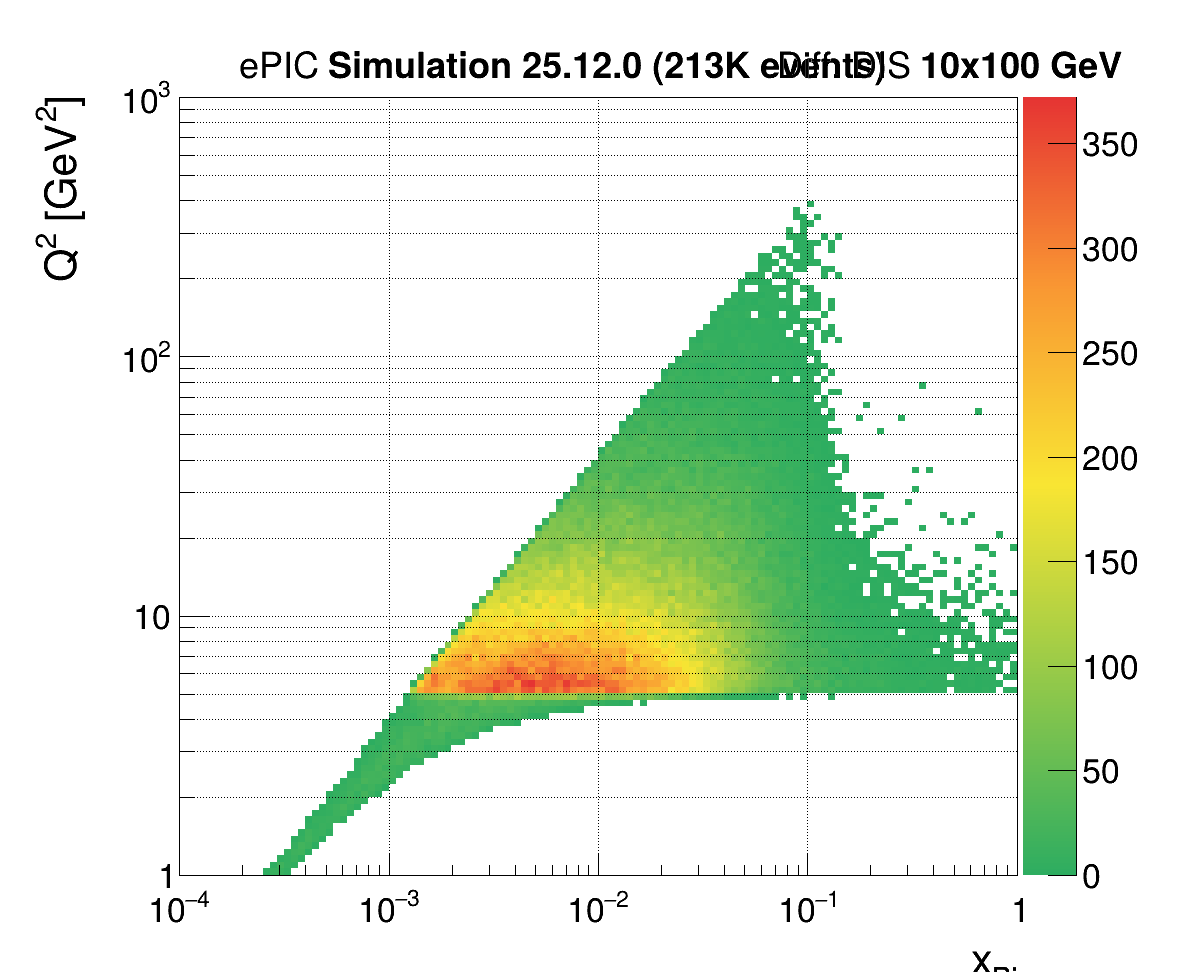
\includegraphics[width=0.6\textwidth]{../figs/inclusive/histos/xbj_q2_density.png}
  \vspace{0.2em}
  \footnotesize
  Event density in $(x_{Bj}, Q^2)$ shows the phase-space coverage.
\end{frame}

\begin{frame}{Diffractive Phase Space I}
  \begin{columns}
    \column{0.5\textwidth}
      \centering
      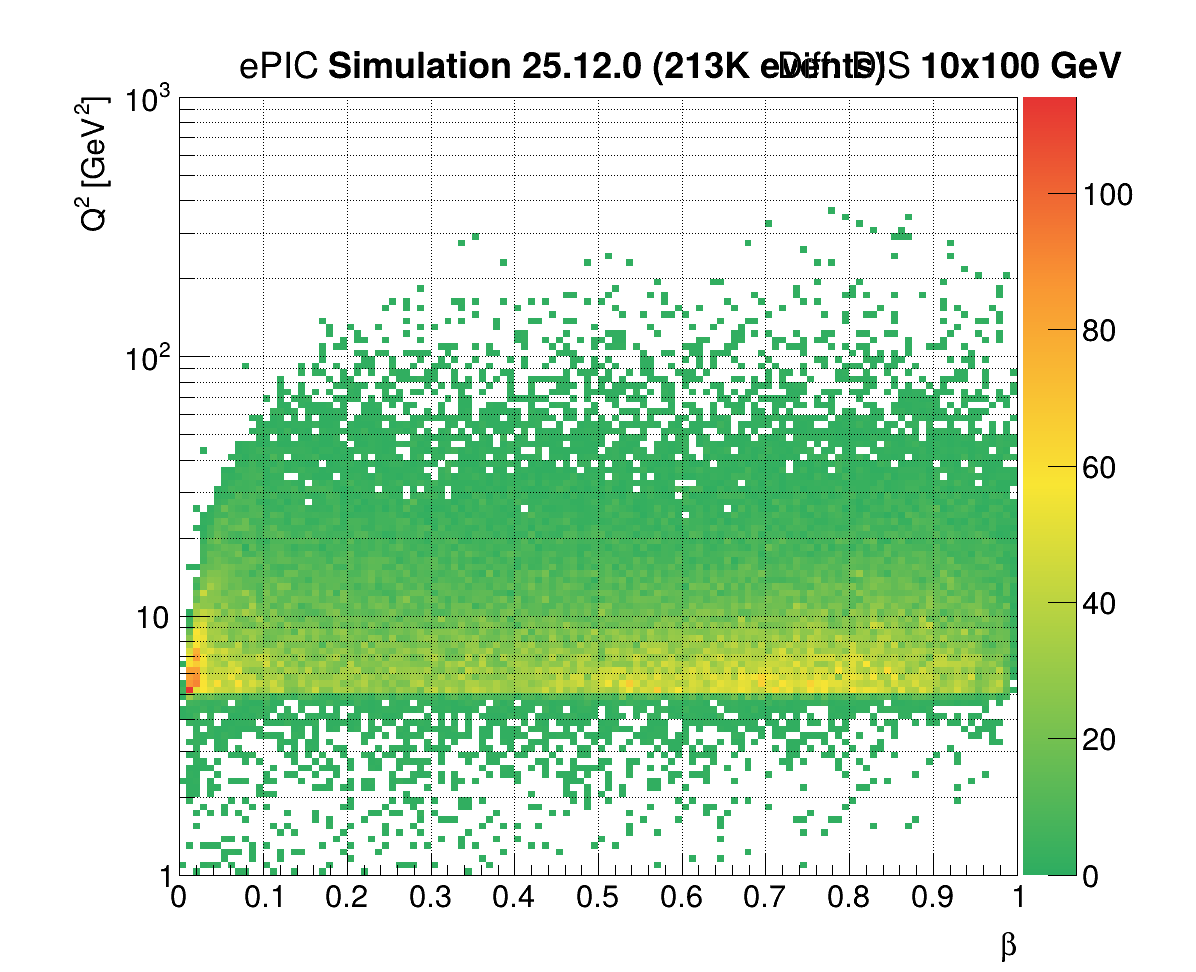
\includegraphics[width=\linewidth]{../figs/diffractive/histos/beta_q2_density.png}
      \footnotesize
      $(\beta, Q^2)$ density.
    \column{0.5\textwidth}
      \centering
      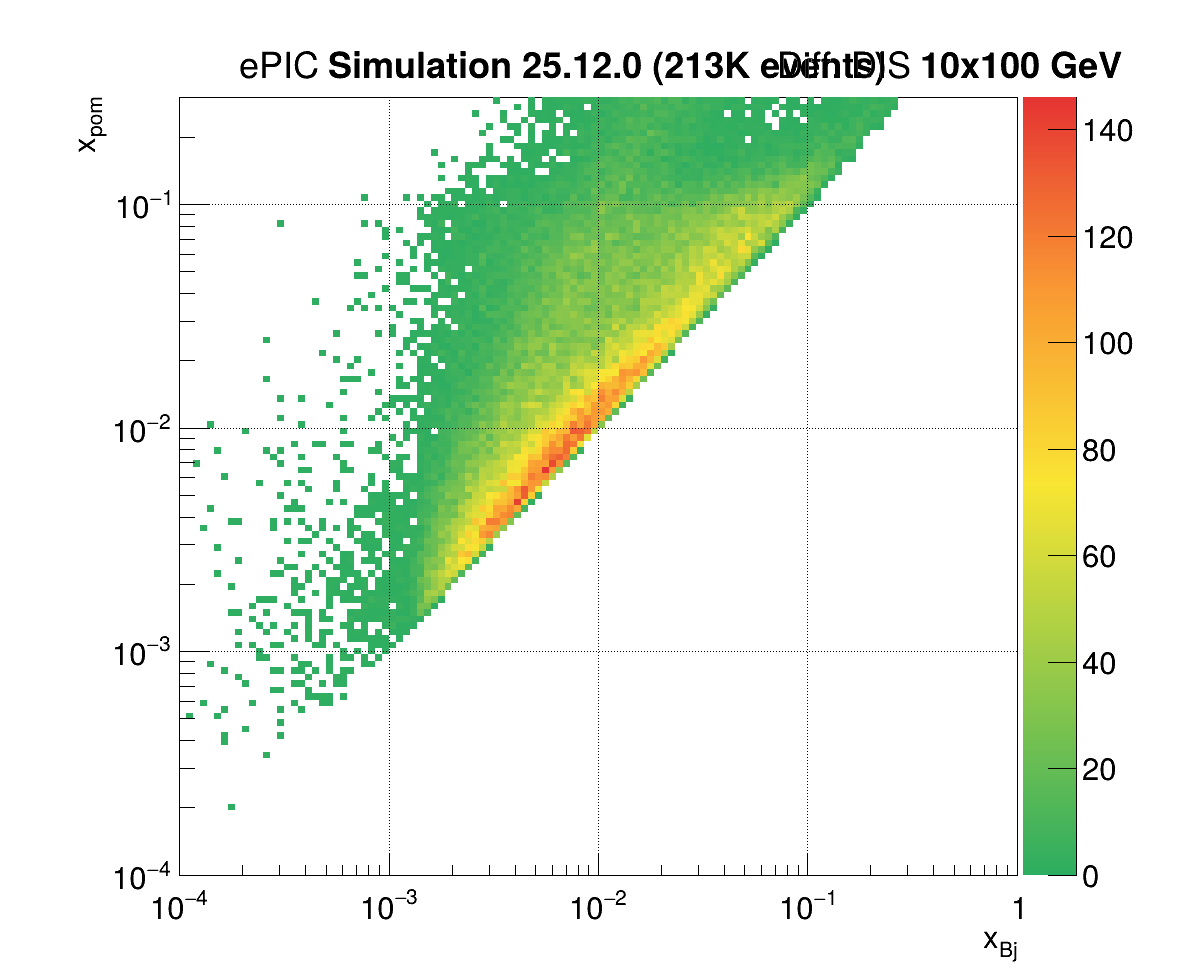
\includegraphics[width=\linewidth]{../figs/diffractive/histos/xbj_xpom_density.png}
      \footnotesize
      $(x_{Bj}, x_{\mathbb{P}})$ density.
  \end{columns}
\end{frame}

\begin{frame}{Diffractive Phase Space II}
  \begin{columns}
    \column{0.5\textwidth}
      \centering
      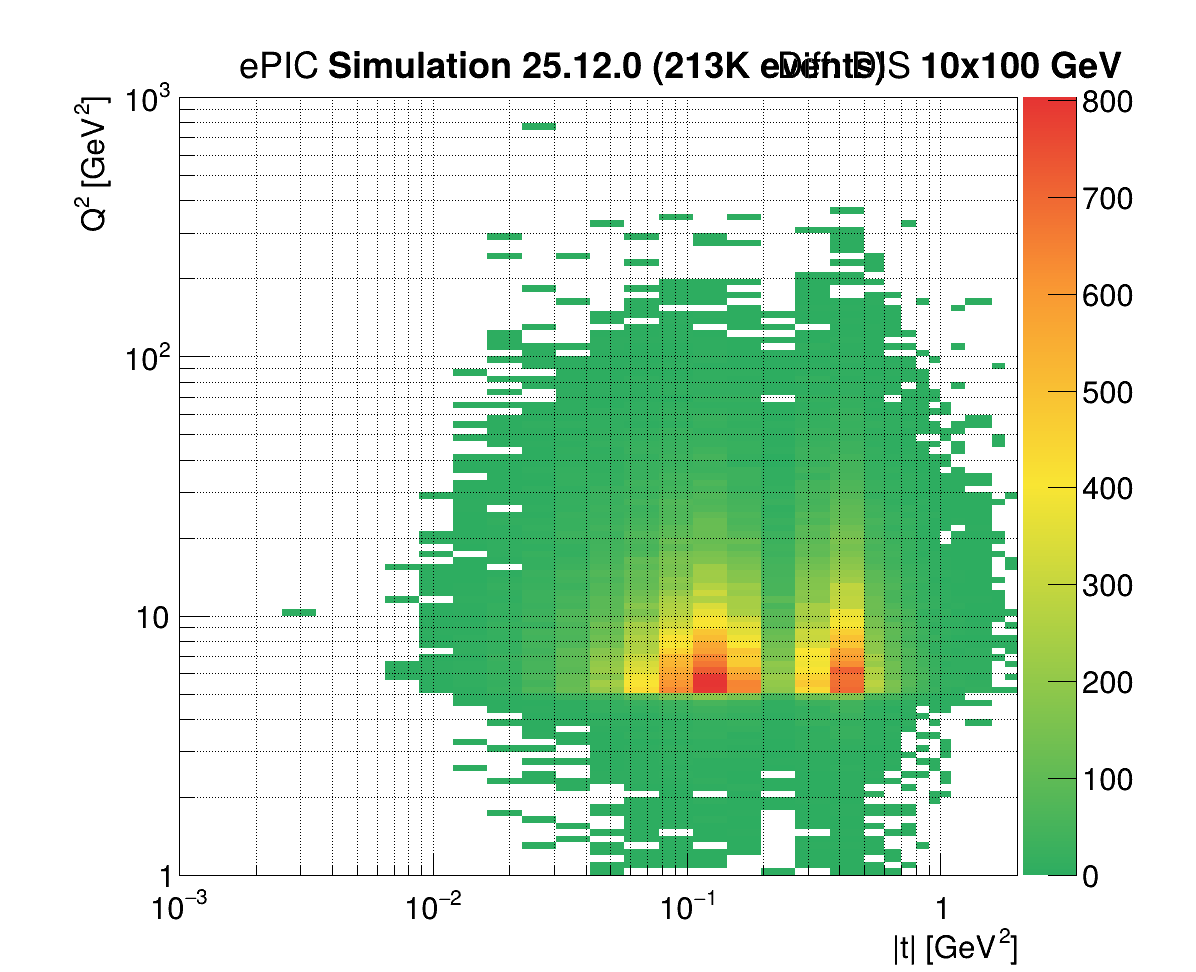
\includegraphics[width=\linewidth]{../figs/diffractive/histos/t_q2_density.png}
      \footnotesize
      $(|t|, Q^2)$ density.
    \column{0.5\textwidth}
      \centering
      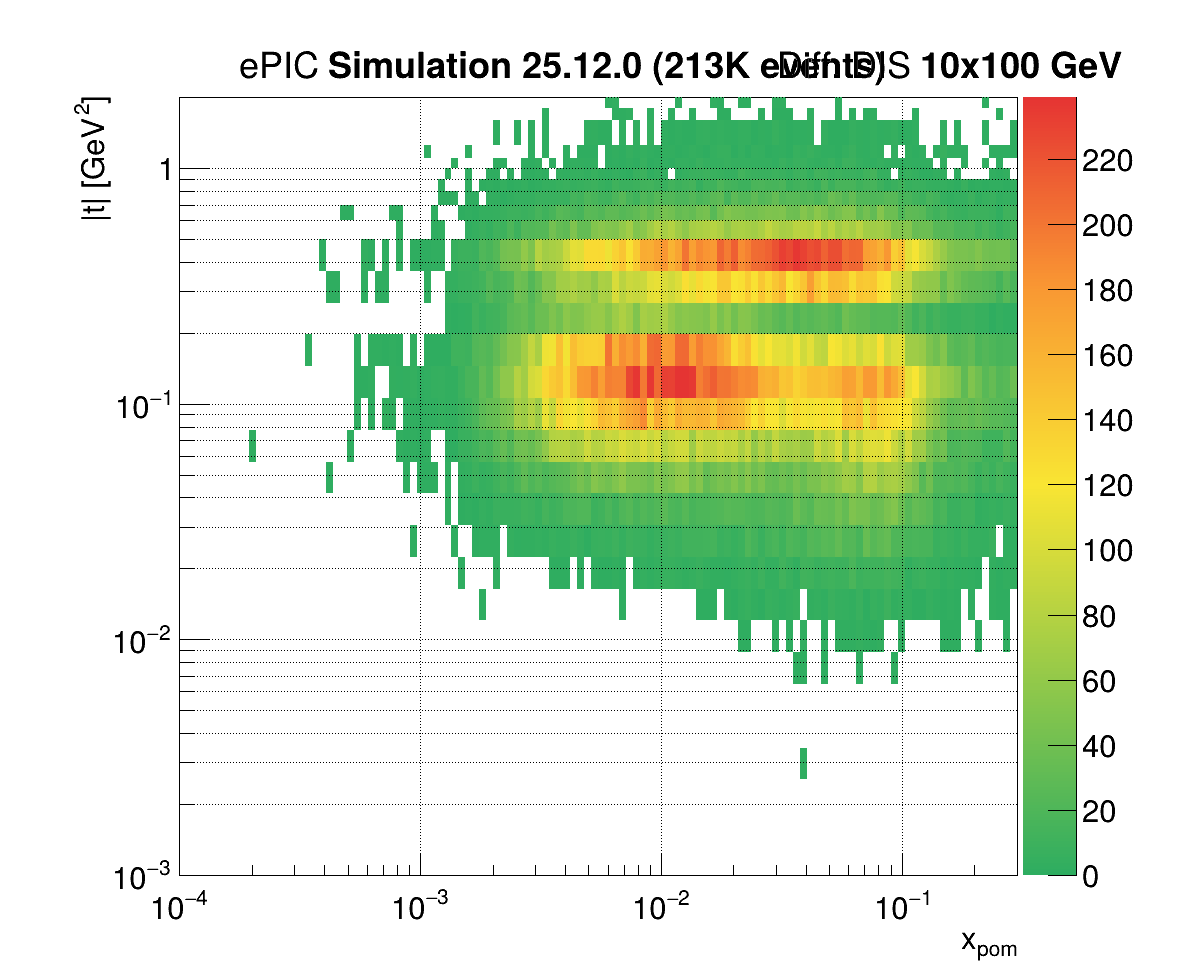
\includegraphics[width=\linewidth]{../figs/diffractive/histos/xpom_t_density.png}
      \footnotesize
      $(x_{\mathbb{P}}, |t|)$ density.
  \end{columns}
\end{frame}

\begin{frame}{Inclusive Kinematics Methods}
  \begin{columns}
    \column{0.5\textwidth}
      \centering
      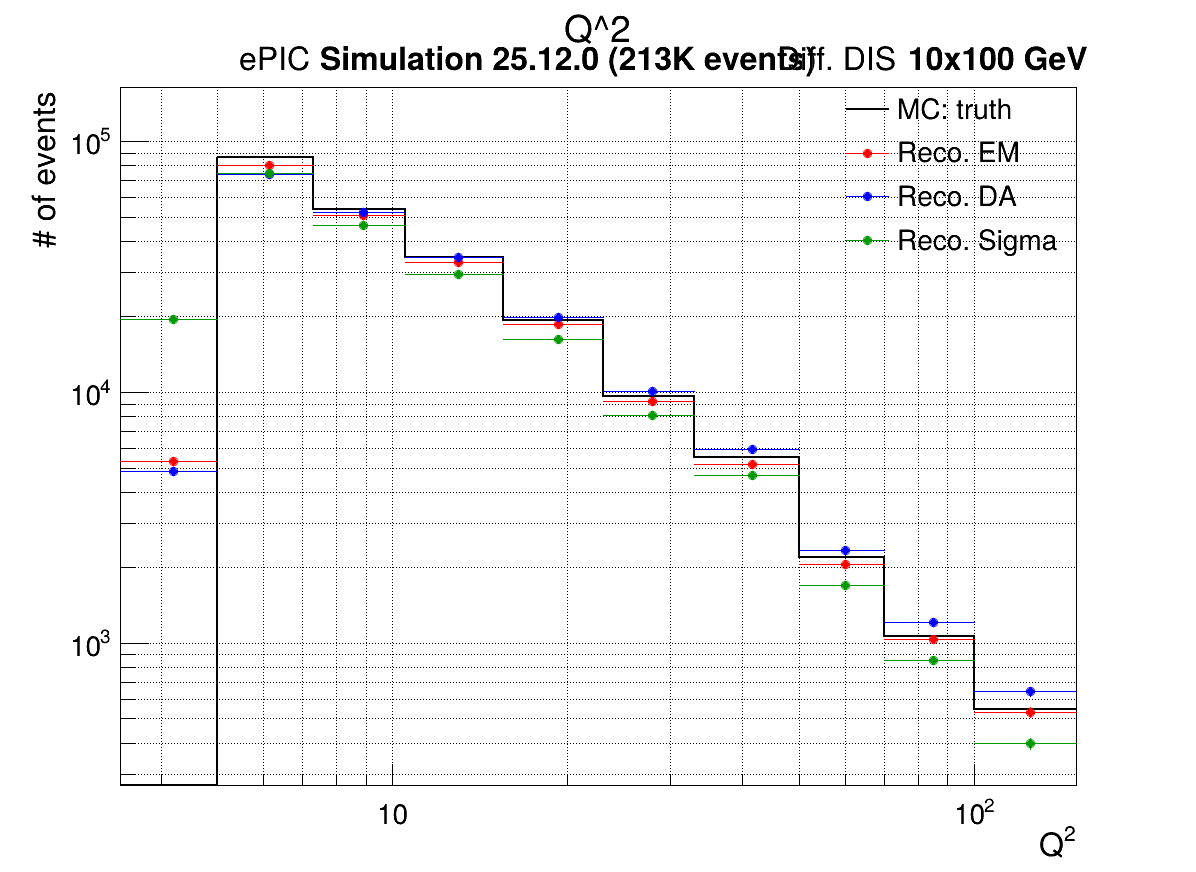
\includegraphics[width=\linewidth]{../figs/inclusive/histos/q2_methods_hist.png}
      \footnotesize
      $Q^2$ reconstructed by EM/DA/Sigma methods.
    \column{0.5\textwidth}
      \centering
      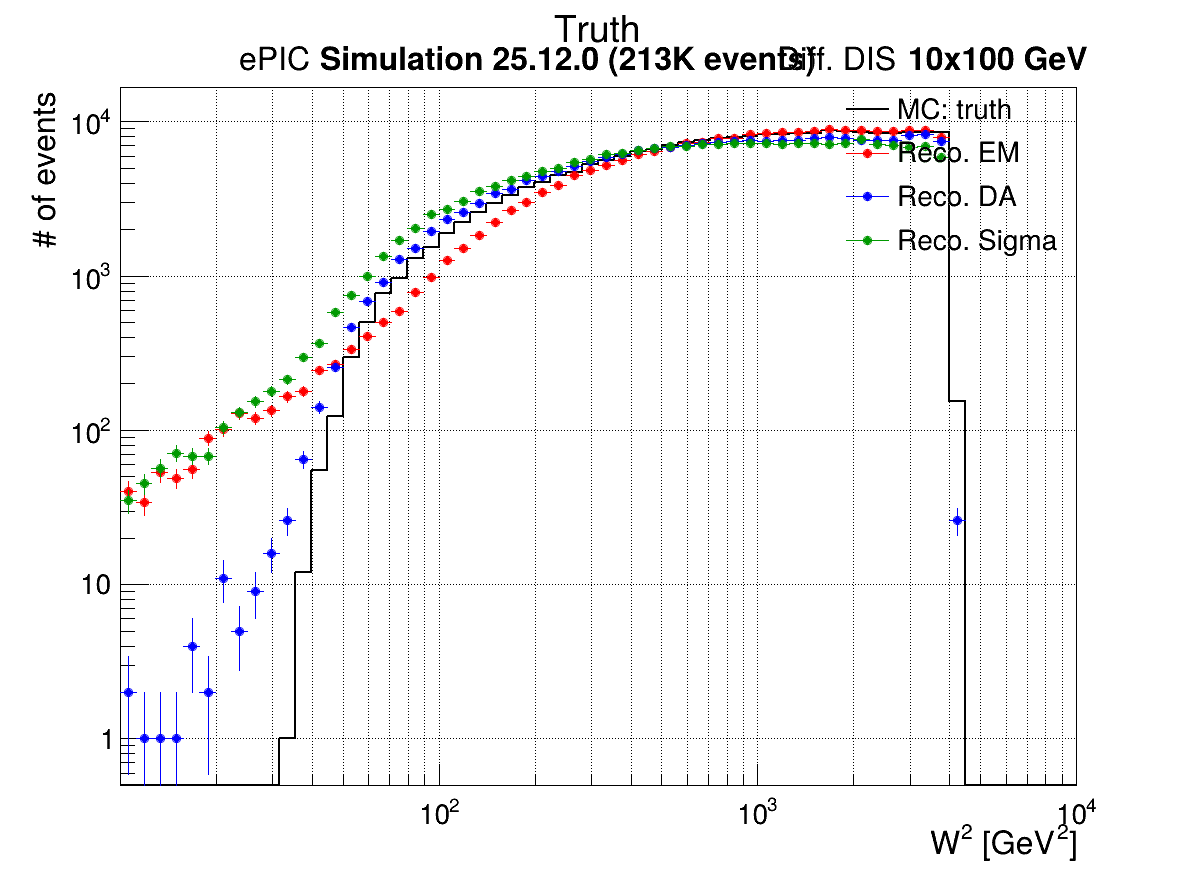
\includegraphics[width=\linewidth]{../figs/inclusive/histos/w2_methods_hist.png}
      \footnotesize
      $W^2$ reconstructed by EM/DA/Sigma methods.
  \end{columns}
\end{frame}

\begin{frame}{Diffractive Definitions}
  \small
  \begin{align*}
    M_X^2 &= \left(\sum_{i \in X} p_i\right)^2 \\
    x_{\mathbb{P}} &= \frac{Q^2 + M_X^2 - t}{Q^2 + W^2 - m_p^2} \\
    \beta &= \frac{x_{Bj}}{x_{\mathbb{P}}} \\
    t &= (p_p - p_p')^2
  \end{align*}
  \vspace{0.4em}
  \footnotesize
  These are computed using the electron method for $Q^2$ and $W^2$ unless noted.
\end{frame}

\begin{frame}{Efficiency Correction (Closure Test)}
  \small
  \begin{itemize}
    \item Split the sample 50/50 into two independent sets (A and B).
    \item Efficiency from MC set A:
      \[
        \epsilon_i = \frac{N^{A}_{\text{reco},i}}{N^{A}_{\text{truth},i}}
      \]
    \item Apply to pseudo-data set B:
      \[
        N^{B}_{\text{corr},i} = \frac{N^{B}_{\text{reco},i}}{\epsilon_i}
      \]
    \item Compare corrected pseudo-data (B) to truth from the same set (B),
          with no acceptance cuts on truth.
  \end{itemize}
\end{frame}

\begin{frame}{Hadronic Mass $M_X^2$}
  \begin{columns}
    \column{0.5\textwidth}
      \centering
      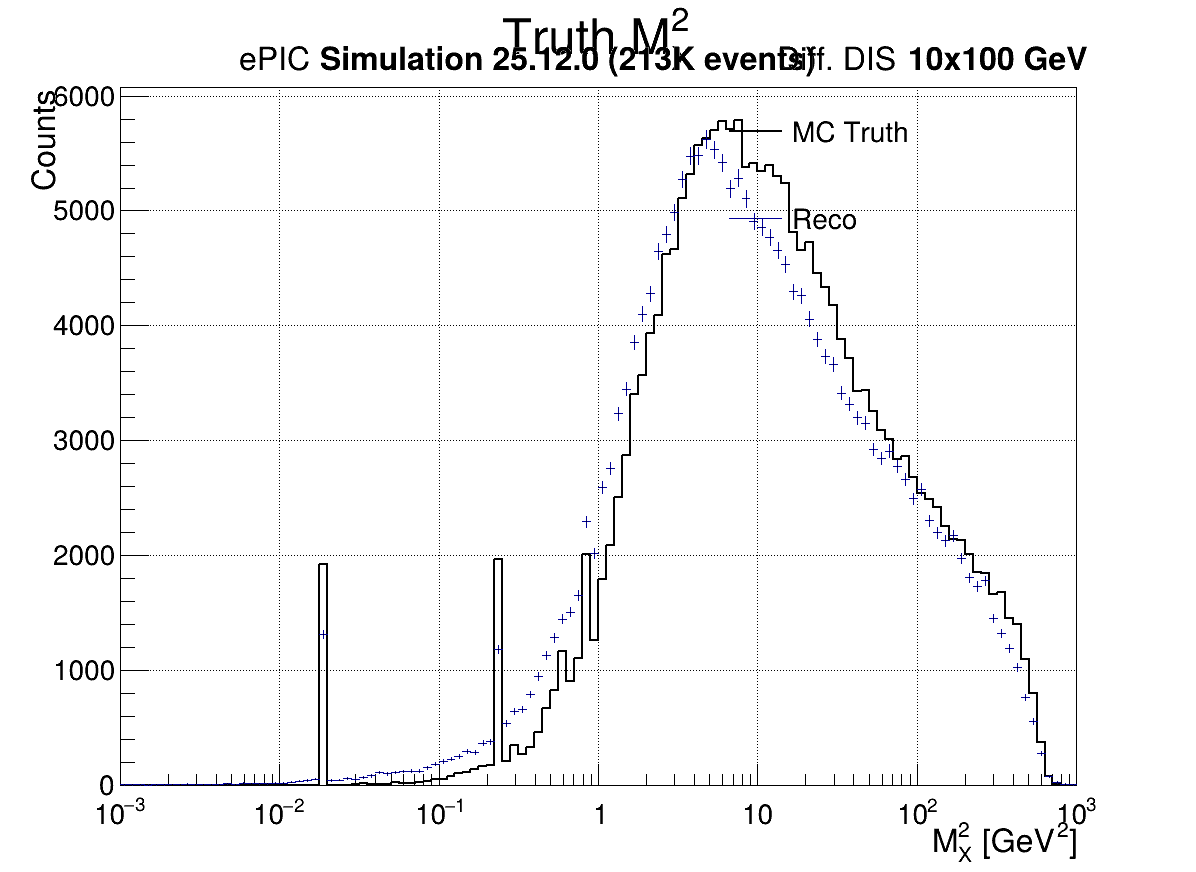
\includegraphics[width=\linewidth]{../figs/diffractive/histos/MX2_comparison.png}
      \footnotesize
      Truth vs reco $M_X^2$ distributions.
    \column{0.5\textwidth}
      \centering
      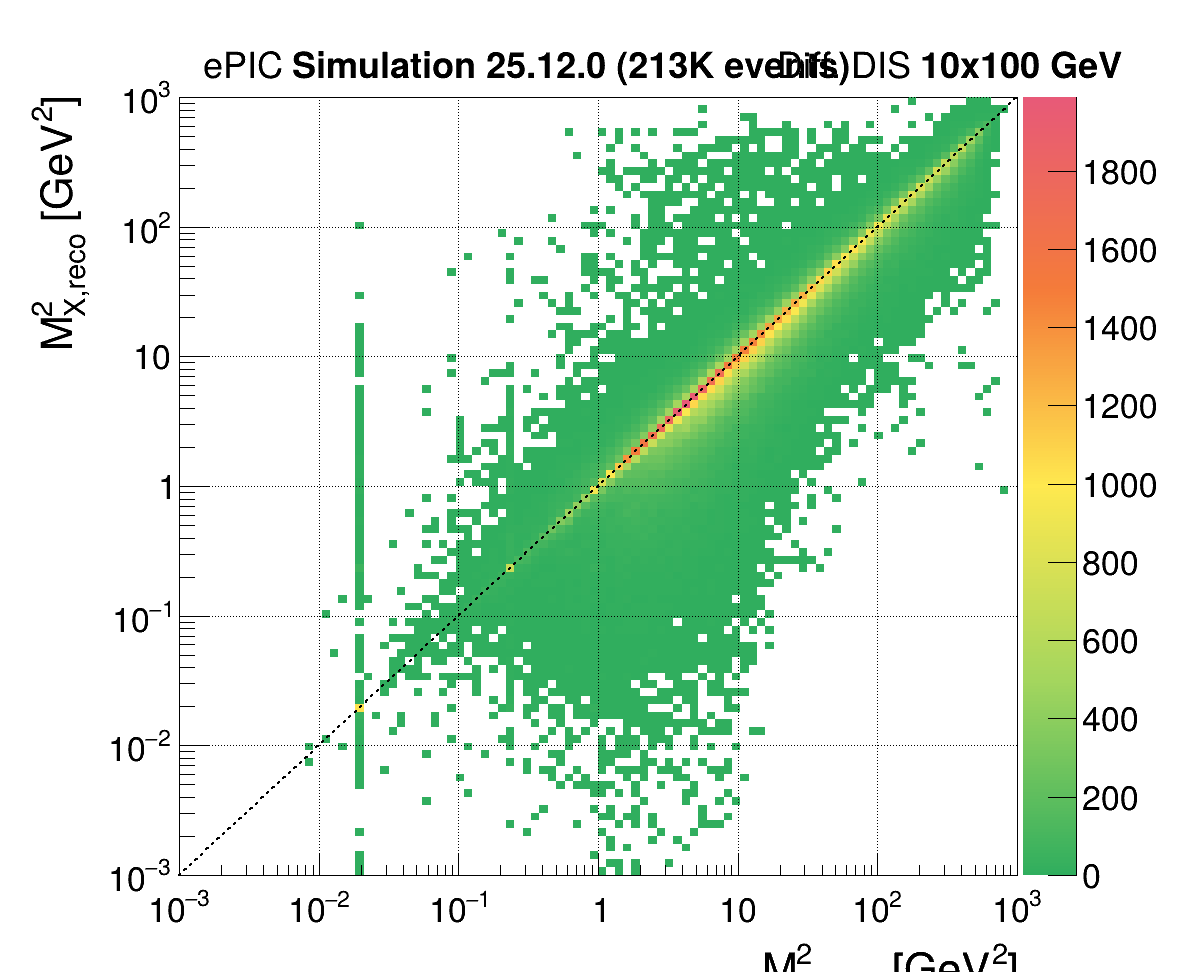
\includegraphics[width=\linewidth]{../figs/diffractive/histos/MX2_corr_unbinned.png}
      \footnotesize
      Unbinned truth vs reco correlation.
  \end{columns}
\end{frame}

\begin{frame}{$x_{\mathbb{P}}$: Uncorrected vs Efficiency-Corrected}
  \begin{columns}
    \column{0.5\textwidth}
      \centering
      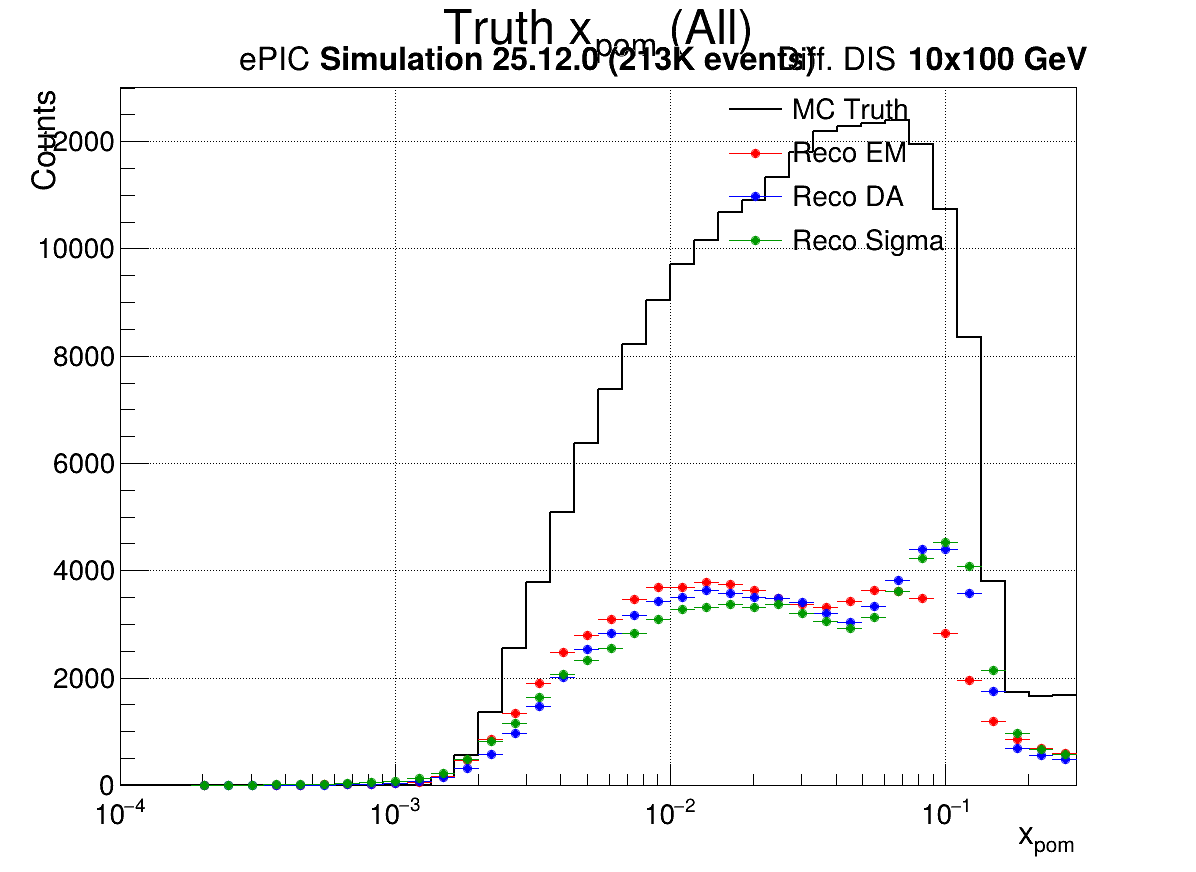
\includegraphics[width=\linewidth]{../figs/diffractive/histos/xpom_def_comparison_all.png}
      \footnotesize
      Uncorrected $x_{\mathbb{P}}$ (truth vs reco).
    \column{0.5\textwidth}
      \centering
      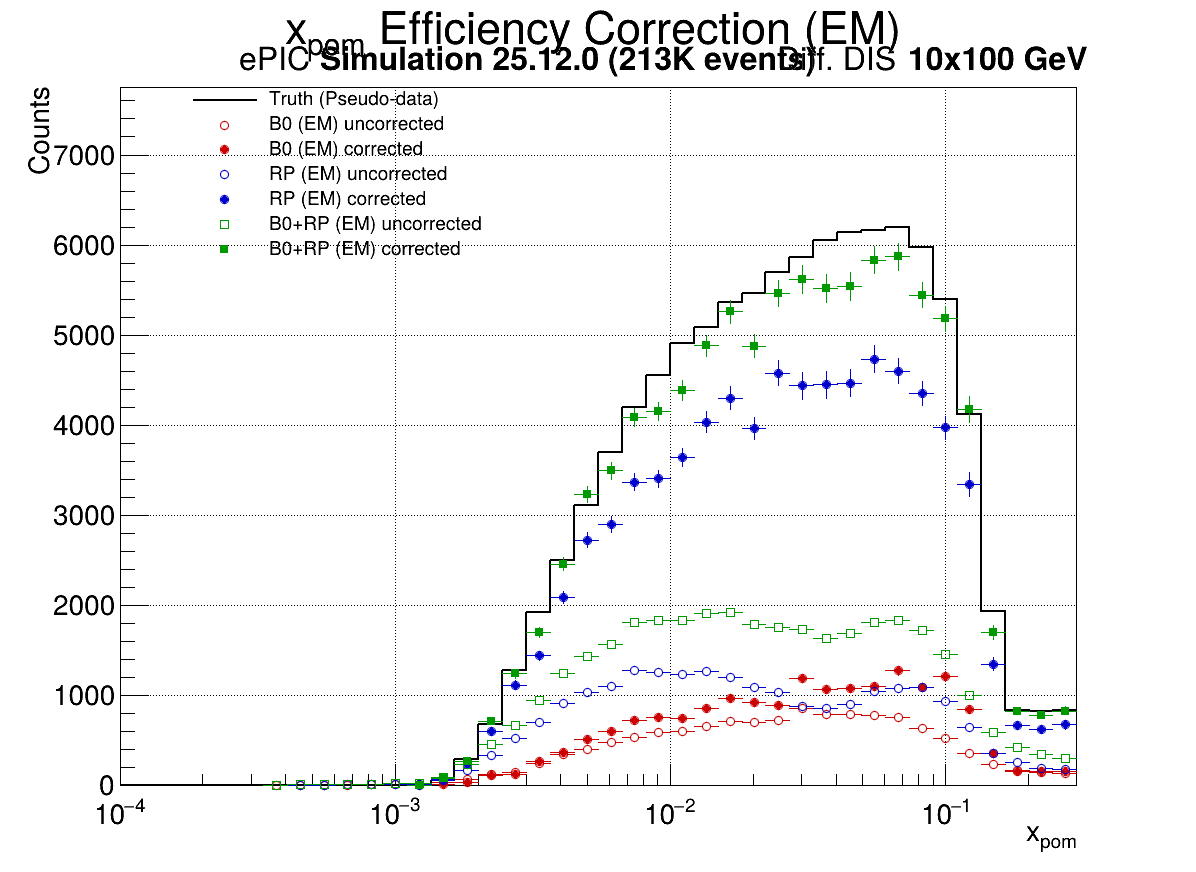
\includegraphics[width=\linewidth]{../figs/diffractive/efficiency/xpom_effcorr.png}
      \footnotesize
      Efficiency-corrected $x_{\mathbb{P}}$ (B0/RP split).
  \end{columns}
\end{frame}

\begin{frame}{$\beta$: Uncorrected vs Efficiency-Corrected}
  \begin{columns}
    \column{0.5\textwidth}
      \centering
      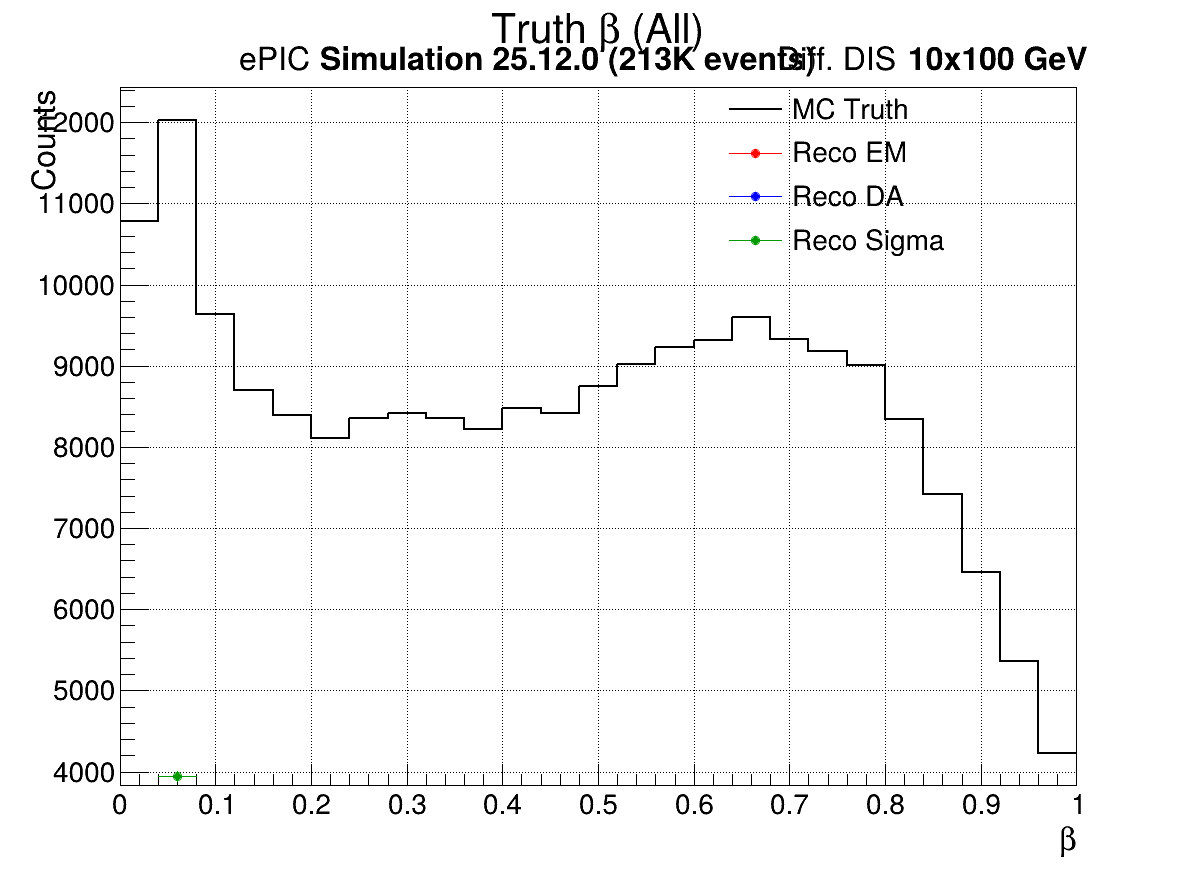
\includegraphics[width=\linewidth]{../figs/diffractive/histos/beta_comparison_all.png}
      \footnotesize
      Uncorrected $\beta$ (truth vs reco).
    \column{0.5\textwidth}
      \centering
      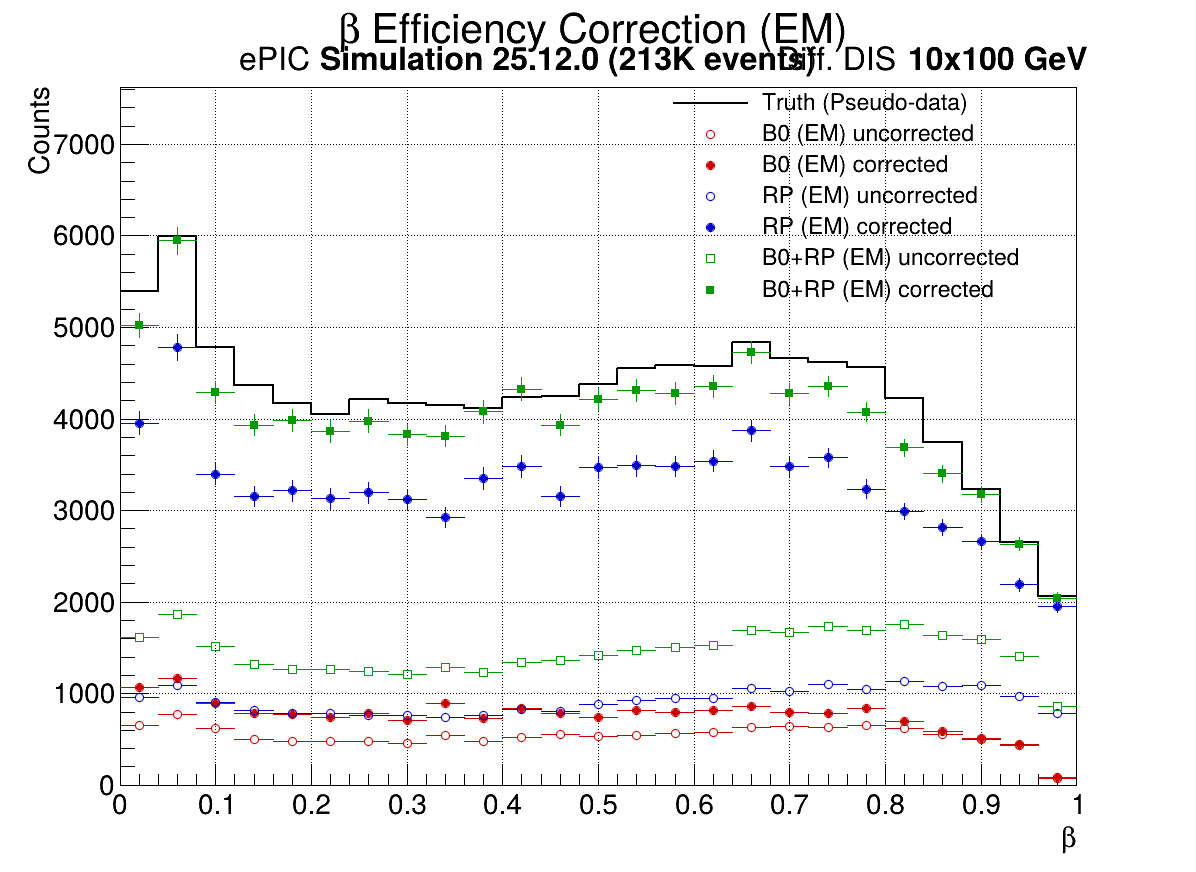
\includegraphics[width=\linewidth]{../figs/diffractive/efficiency/beta_effcorr.png}
      \footnotesize
      Efficiency-corrected $\beta$ (B0/RP split).
  \end{columns}
  \vspace{0.2em}
  \footnotesize
  Efficiency: $\epsilon = N_{\text{reco}}/N_{\text{truth}}$, corrected pseudo-data: $N_{\text{corr}} = N_{\text{pdata}}/\epsilon$.
\end{frame}

\begin{frame}{Proton-Tagged Closure Test: $|t|$ and $\theta$}
  \begin{columns}
    \column{0.5\textwidth}
      \centering
      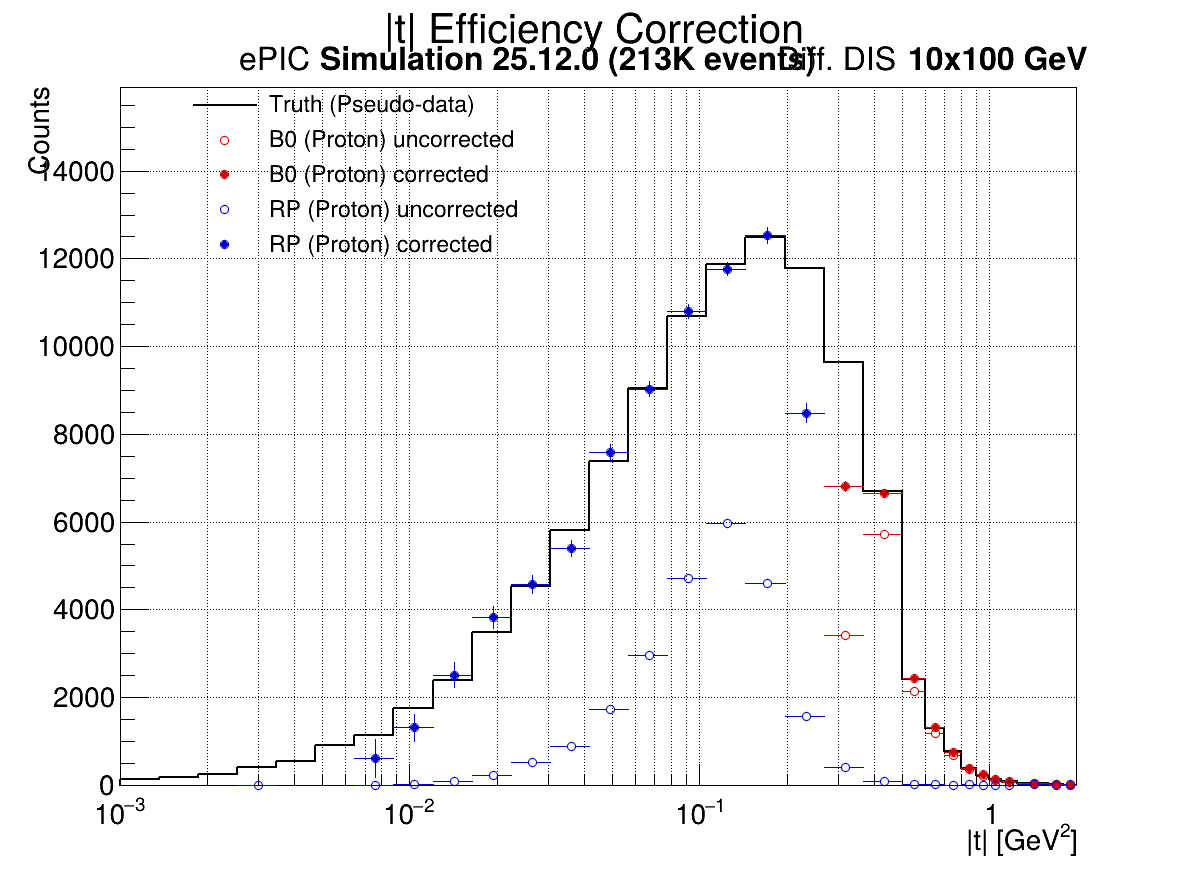
\includegraphics[width=\linewidth]{../figs/diffractive/efficiency/t_effcorr.png}
      \footnotesize
      $|t|$ closure test (B0 vs RP).
    \column{0.5\textwidth}
      \centering
      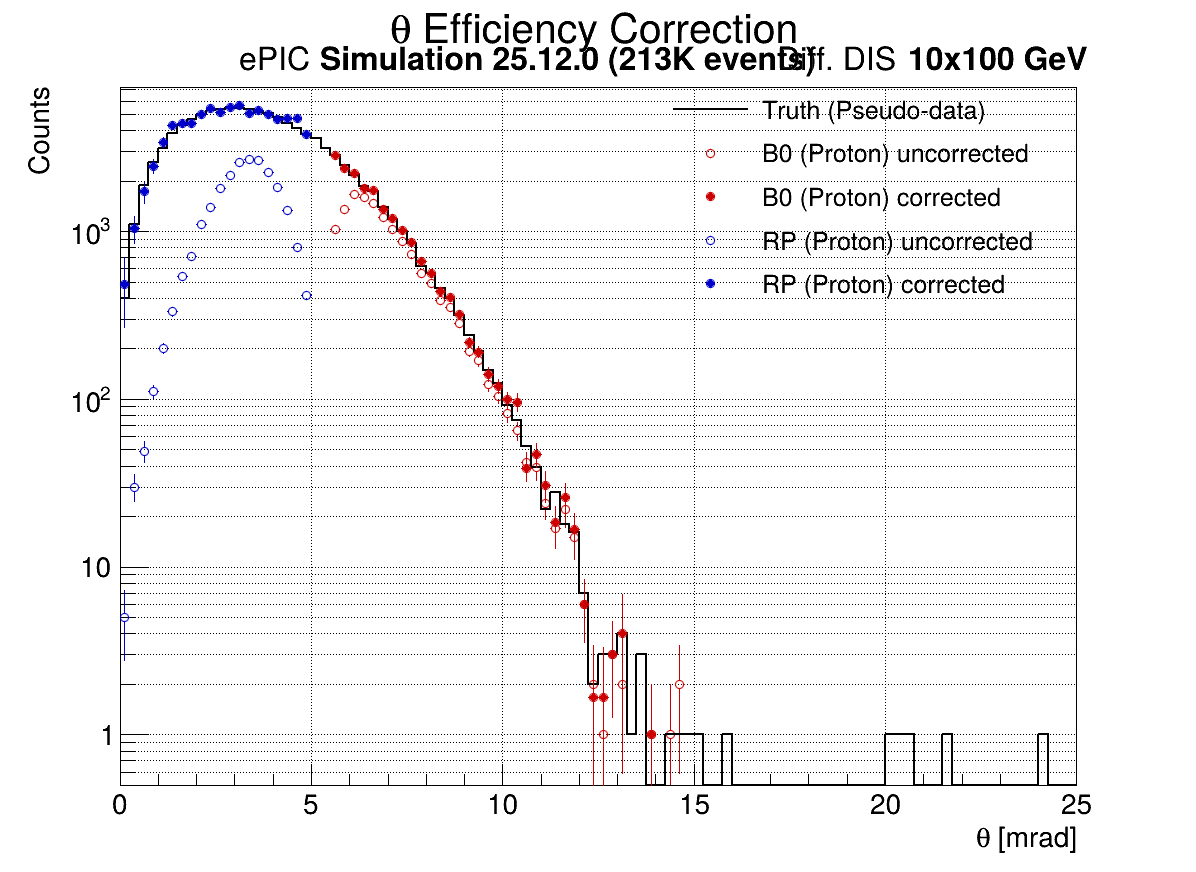
\includegraphics[width=\linewidth]{../figs/diffractive/efficiency/theta_effcorr.png}
      \footnotesize
      Proton scattering angle $\theta$ (log-$y$).
  \end{columns}
\end{frame}

\begin{frame}{$x_{\mathbb{P}}$ Correlations (EM)}
  \begin{columns}
    \column{0.5\textwidth}
      \centering
      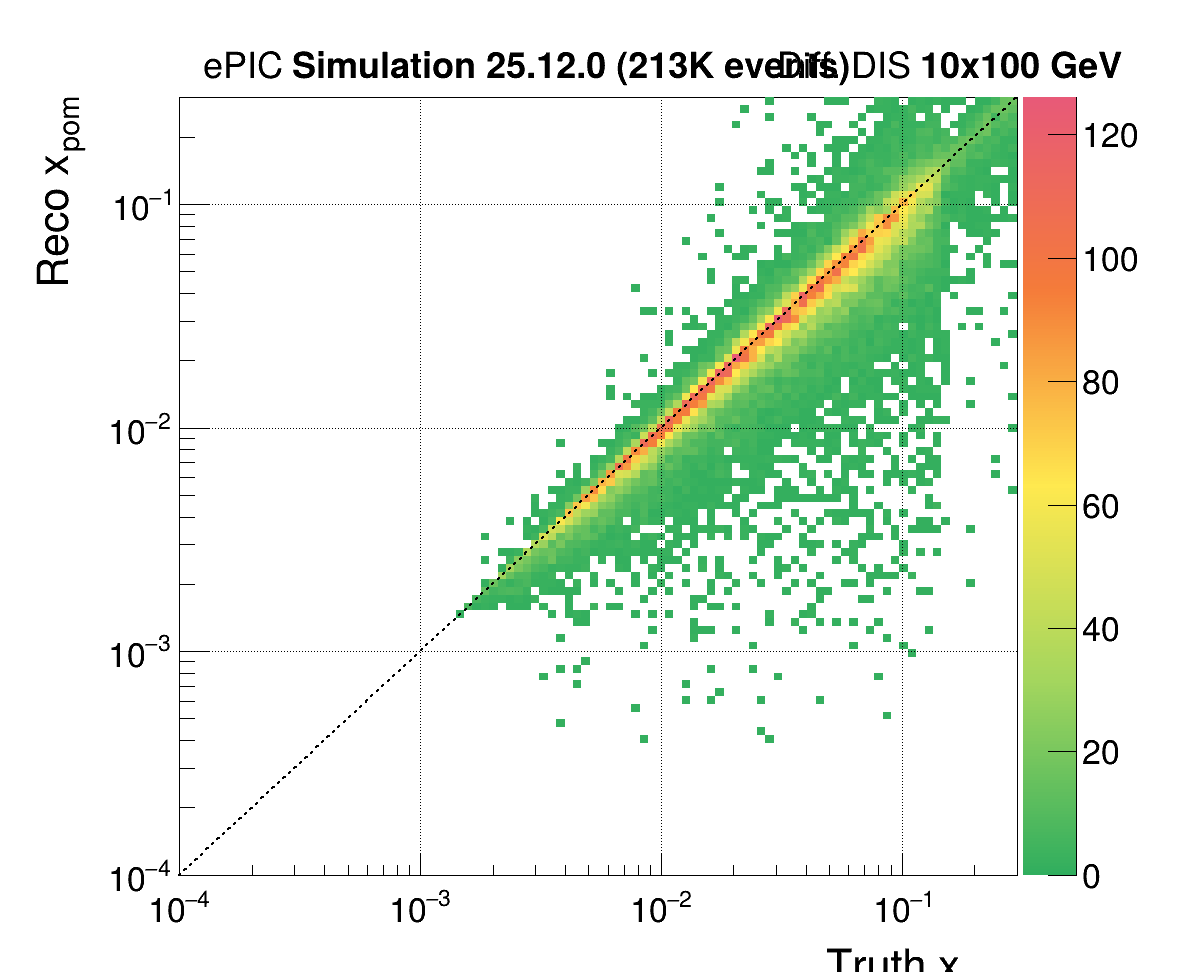
\includegraphics[width=\linewidth]{../figs/diffractive/histos/xpom_corr_unbinned_em_b0.png}
      \footnotesize
      Truth vs reco $x_{\mathbb{P}}$ (B0).
    \column{0.5\textwidth}
      \centering
      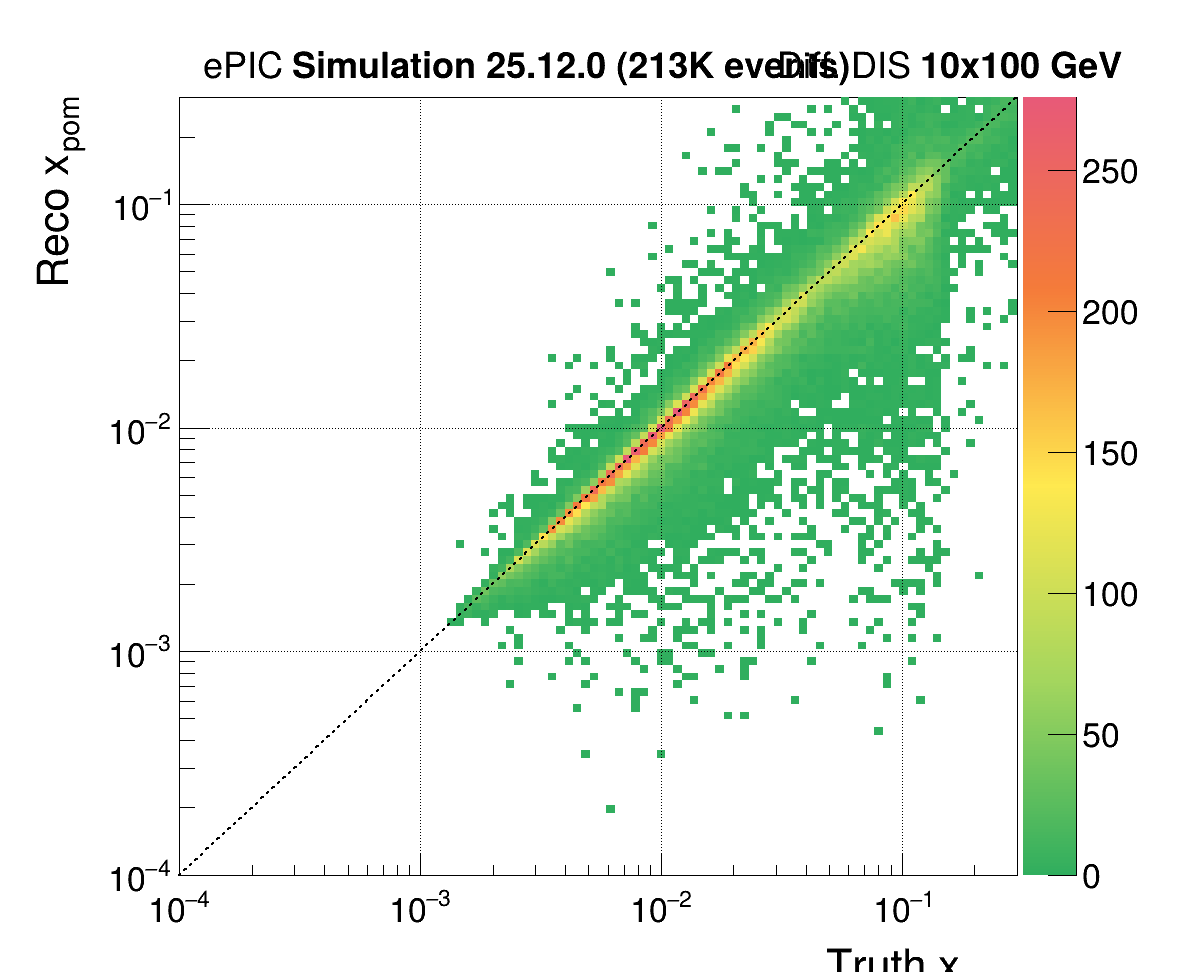
\includegraphics[width=\linewidth]{../figs/diffractive/histos/xpom_corr_unbinned_em_rp.png}
      \footnotesize
      Truth vs reco $x_{\mathbb{P}}$ (RP).
  \end{columns}
\end{frame}

\begin{frame}{$\beta$ Correlations (EM)}
  \begin{columns}
    \column{0.5\textwidth}
      \centering
      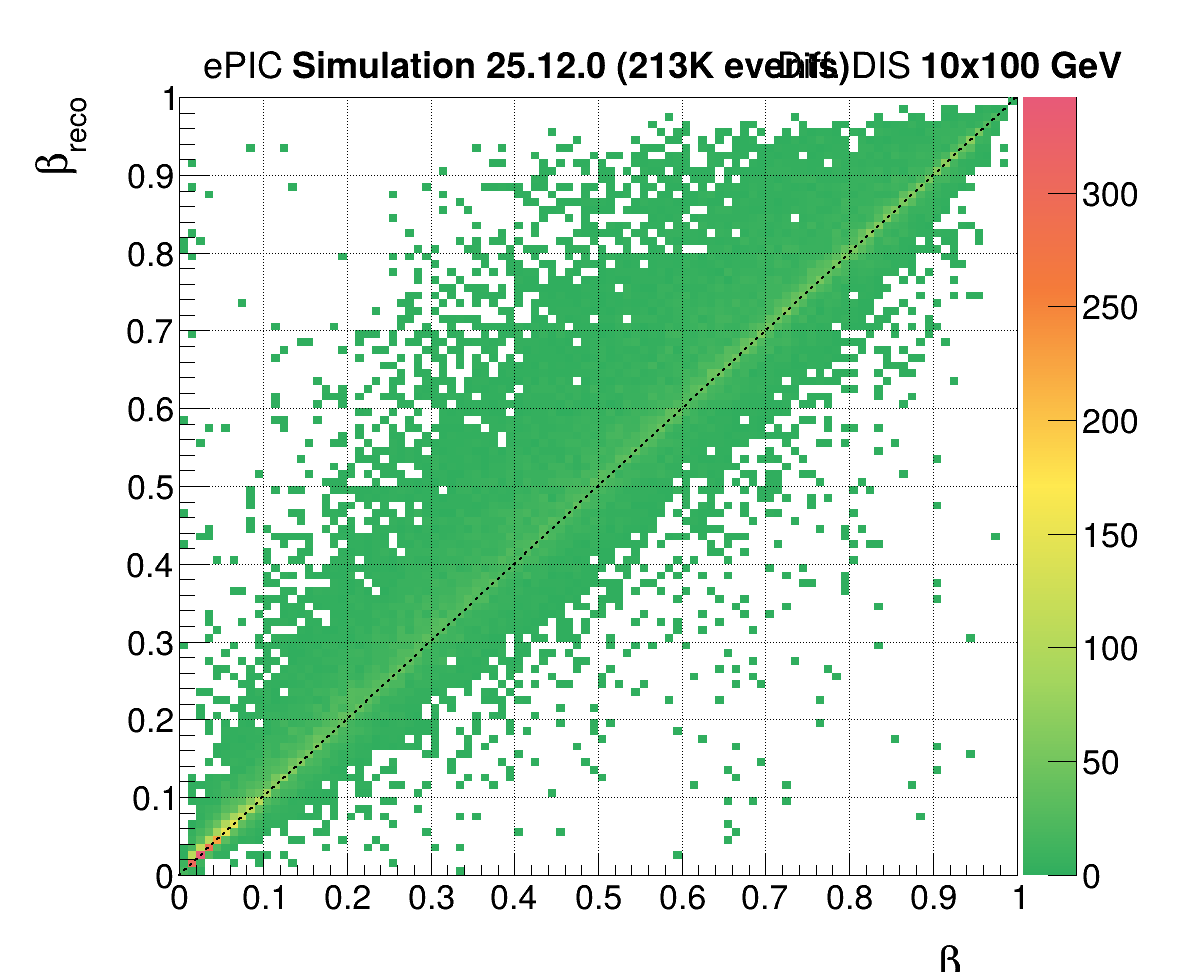
\includegraphics[width=\linewidth]{../figs/diffractive/histos/beta_corr_unbinned_em_b0.png}
      \footnotesize
      Truth vs reco $\beta$ (B0).
    \column{0.5\textwidth}
      \centering
      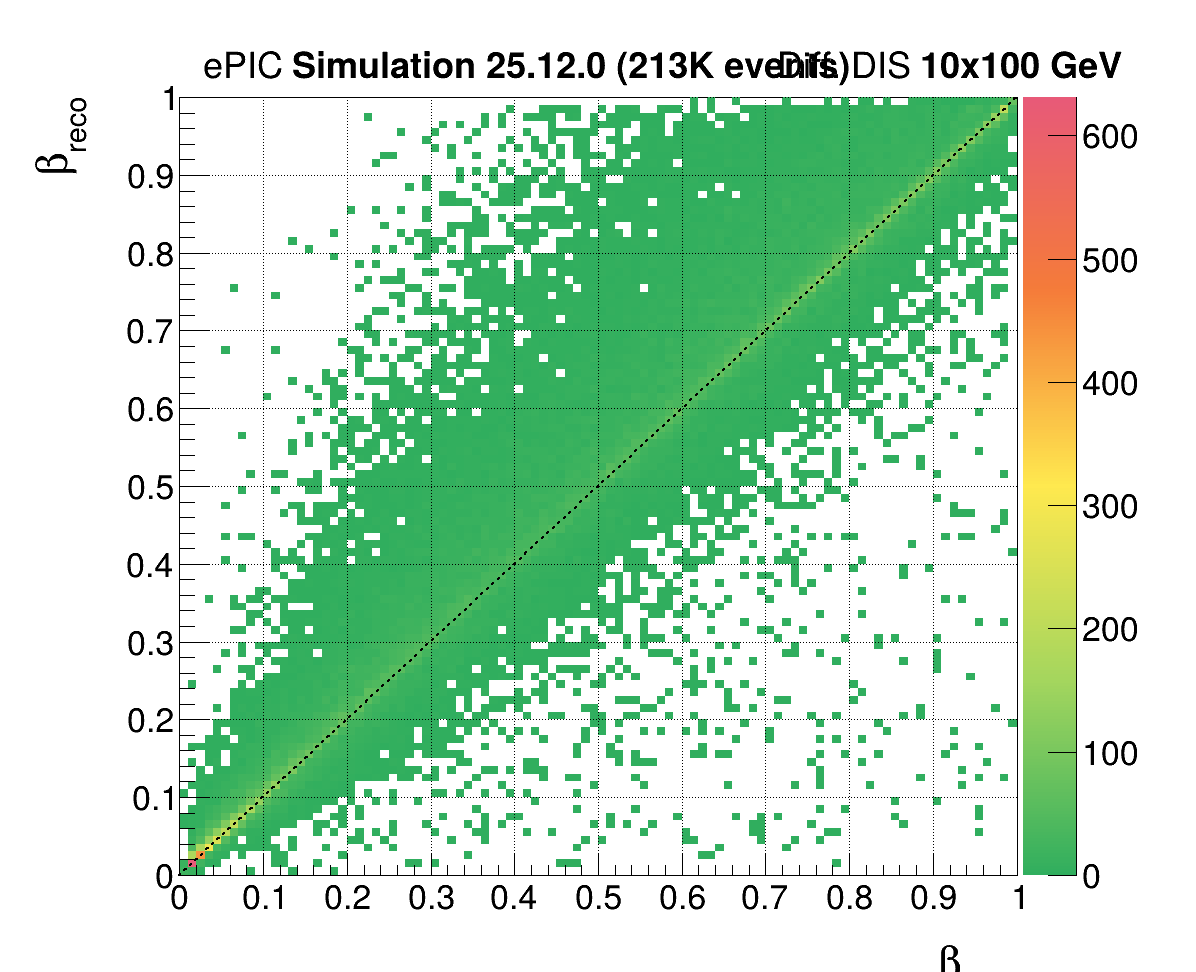
\includegraphics[width=\linewidth]{../figs/diffractive/histos/beta_corr_unbinned_em_rp.png}
      \footnotesize
      Truth vs reco $\beta$ (RP).
  \end{columns}
\end{frame}



%\begin{frame}{$x_{\mathbb{P}}$ Response Matrices (EM)}
%  \begin{columns}
%    \column{0.5\textwidth}
%      \centering
%      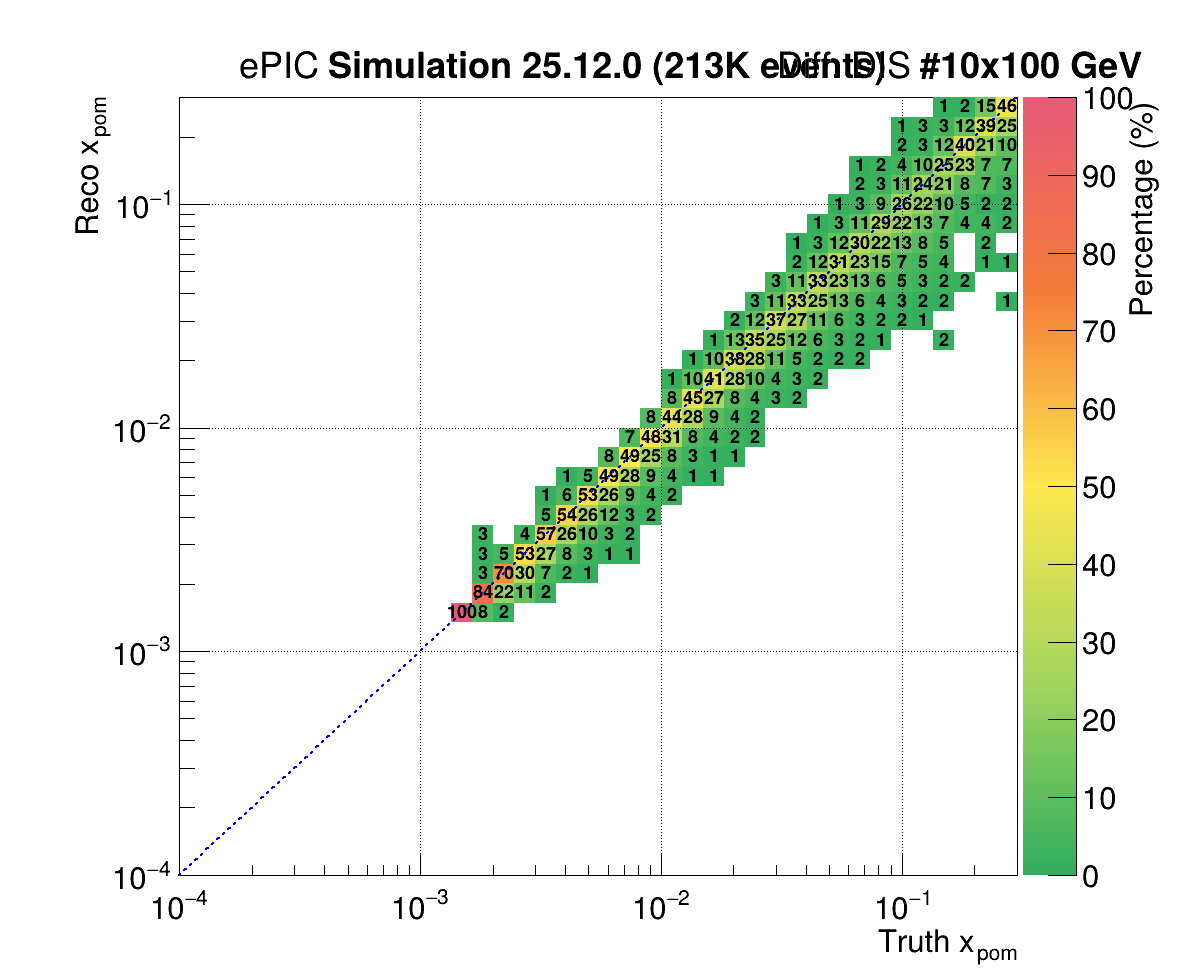
\includegraphics[width=\linewidth]{../figs/diffractive/response/response_xpom_em_b0.png}
%      \footnotesize
%      $x_{\mathbb{P}}$ response (B0).
%    \column{0.5\textwidth}
%      \centering
%      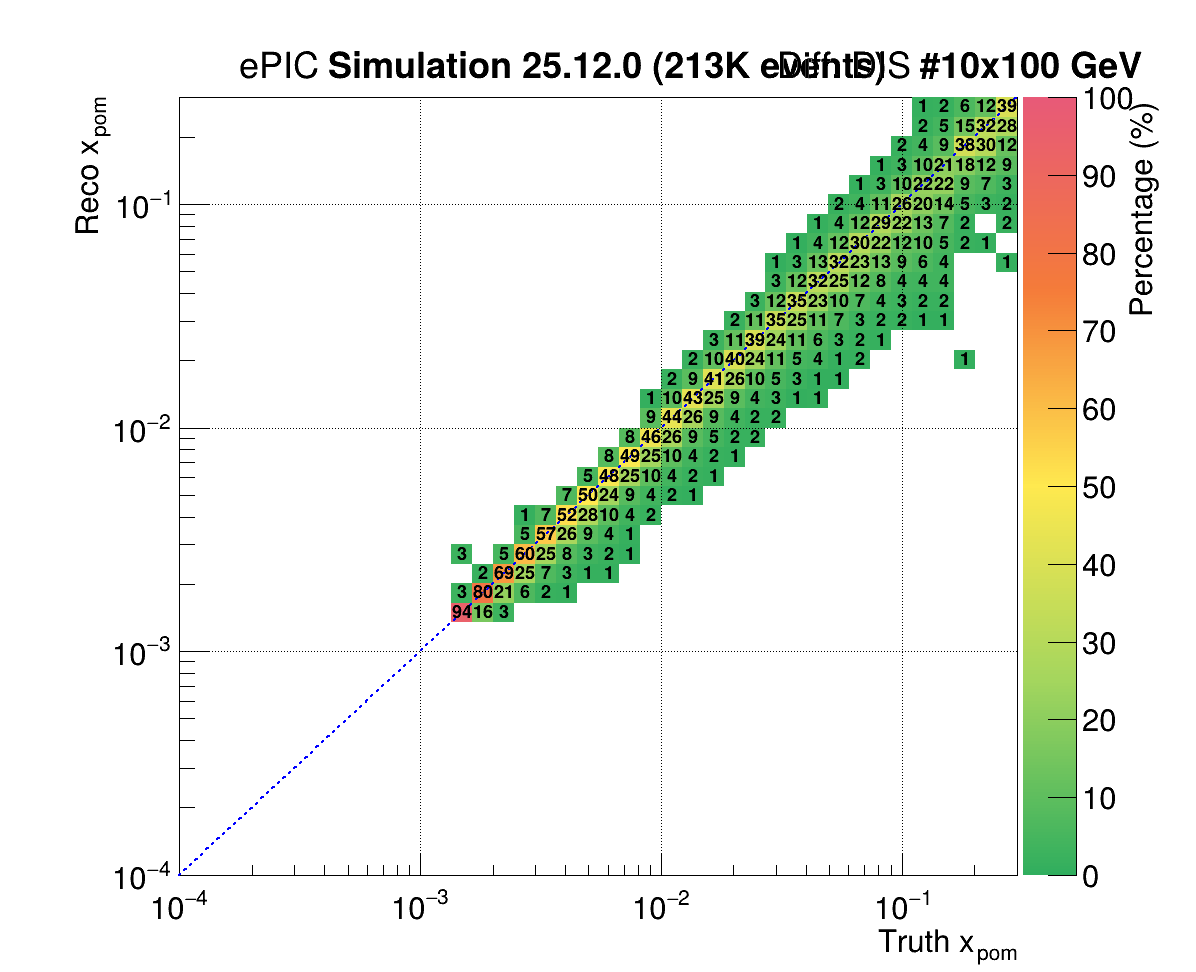
\includegraphics[width=\linewidth]{../figs/diffractive/response/response_xpom_em_rp.png}
%      \footnotesize
%      $x_{\mathbb{P}}$ response (RP).
%  \end{columns}
%\end{frame}

\begin{frame}{$\beta$ Response Matrices (EM)}
  \begin{columns}
    \column{0.5\textwidth}
      \centering
      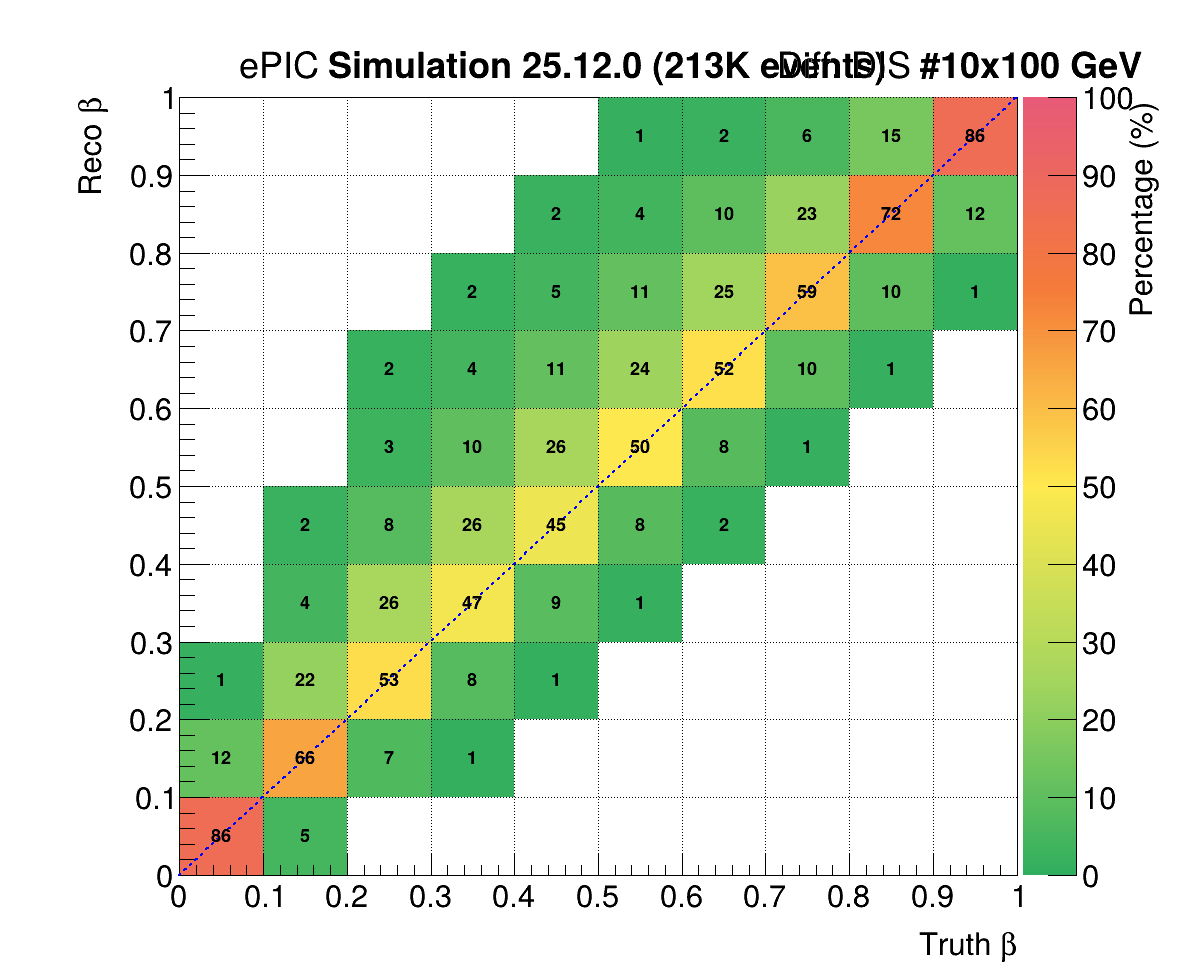
\includegraphics[width=\linewidth]{../figs/diffractive/response/response_beta_em_b0.png}
      \footnotesize
      $\beta$ response (B0).
    \column{0.5\textwidth}
      \centering
      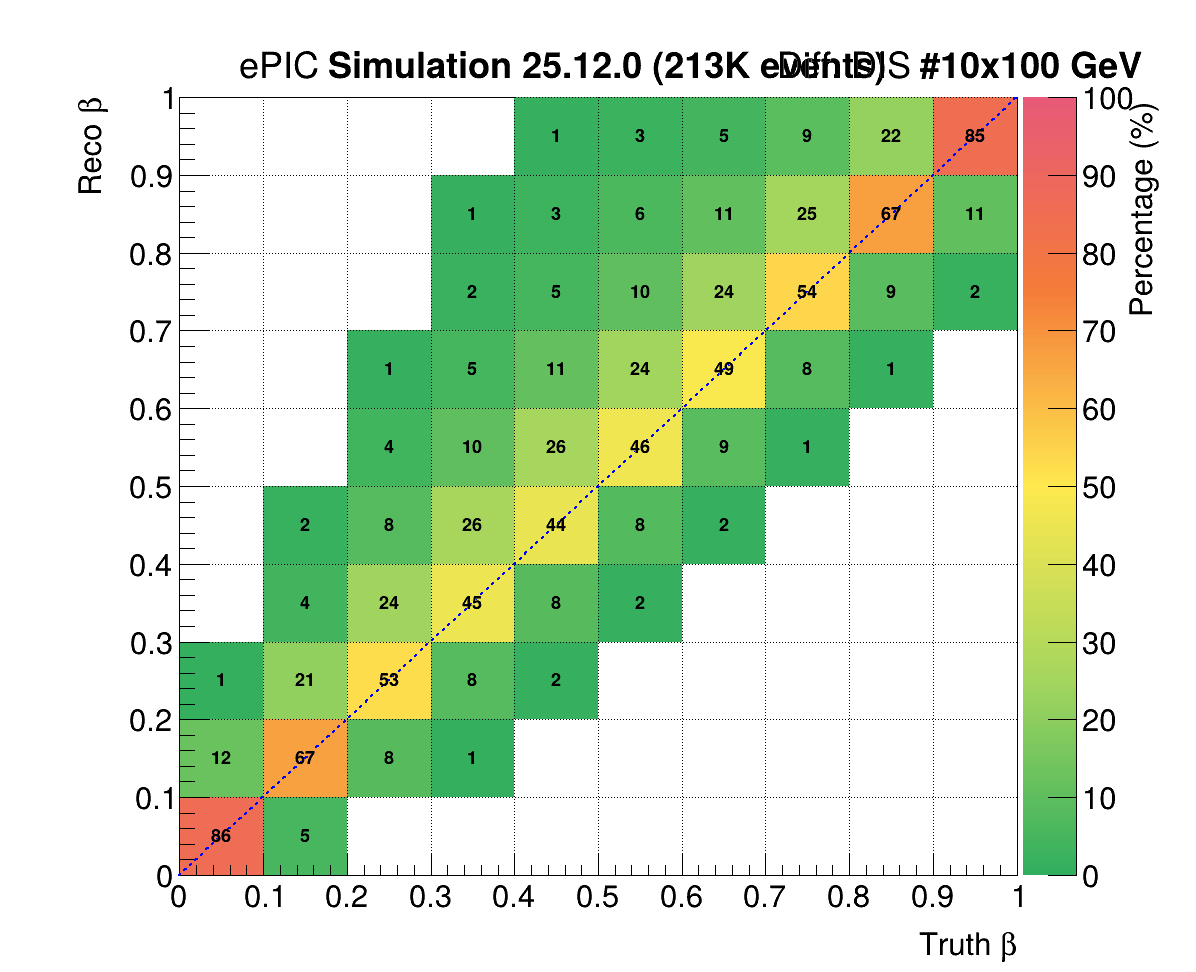
\includegraphics[width=\linewidth]{../figs/diffractive/response/response_beta_em_rp.png}
      \footnotesize
      $\beta$ response (RP).
  \end{columns}
\end{frame}

%\begin{frame}{$|t|$ Response Matrices}
  %\begin{columns}
    %\column{0.5\textwidth}
      %\centering
      %\includegraphics[width=\linewidth]{%../figs/diffractive/response/respon%se_t_b0.png}
    %  \footnotesize
    %  $|t|$ response (B0).
    %\column{0.5\textwidth}
      %\centering
      %\includegraphics[width=\linewidth]{%../figs/diffractive/response/respon%se_t_rp.png}
   %   \footnotesize
  %    $|t|$ response (RP).
 % \end{columns}
%\end{frame}

\begin{frame}{Summary}
  \begin{itemize}
    \item Inclusive and diffractive observables show expected phase-space coverage.
    \item Proton-tagged (B0/RP) closure tests diagnose acceptance effects.
    \item Efficiency-corrected pseudo-data trends toward truth in most regions.
  \end{itemize}
\end{frame}

\begin{frame}{Plot Coverage}
  \small
  \begin{itemize}
    \item Included: inclusive $(x_{Bj},Q^2)$ density, $Q^2/W^2/x_{Bj}/y$ method comparisons,
          and inclusive efficiency-correction plots.
    \item Included: diffractive $M_X^2$, $x_{\mathbb{P}}$, $\beta$ histograms and
          truth-vs-reco correlations, plus key density plots.
    \item Included: B0/RP efficiency-correction closure plots for $x_{\mathbb{P}}$, $\beta$, $|t|$, and $\theta$.
    \item Included: diffractive response matrices and unbinned correlations (EM shown for B0/RP).
    \item Additional plots live in \texttt{figs/} and can be added in an appendix on request.
  \end{itemize}
\end{frame}

\end{document}
